% Change-marked copy for review: text added or changed after the annotated
% draft is in red. Do NOT submit this file; submit isbi2027_overleaf.tex.
\documentclass{article}
\usepackage{spconf,amsmath,amssymb,graphicx}
\usepackage{booktabs}
\usepackage{cite}
\usepackage{url}
\usepackage{xcolor}
\definecolor{RED}{rgb}{1,0,0}
\graphicspath{{figures/}{./}}

% Values still to be filled in by the authors are marked in red; remove before submission.
\newcommand{\tbd}[1]{\textcolor{red}{#1}}

\title{\textcolor{red}{Multi-Representation Anchored Flow Matching}\\
\textcolor{red}{for EEG Spatial Super-Resolution}}
\name{Author Name(s)}
\address{Indian Institute of Technology Mandi\\
Mandi, Himachal Pradesh, India\\
email@example.com}

\begin{document}
\maketitle

\begin{abstract}
EEG \textcolor{red}{spatial super-resolution (SR) estimates the signals of unrecorded
electrodes from the recorded ones, enabling low-density headsets and the
repair of failed channels. Spherical-spline interpolation is the standard
method,} and deep generative models have recently been proposed as an
alternative. We evaluate graph-informed flow matching (GiFlow) for
\textcolor{red}{recovering} 50\% of the electrodes in participants unseen during training.
With its published hyperparameters, our implementation is substantially
less accurate than the spline on \textcolor{red}{the SEED-IV dataset} (normalized
mean-squared error, NMSE, 0.335 vs 0.150). We attribute this to the
training mask, the heat-kernel source of the flow and rapid overfitting,
and address each. The resulting model, which initializes the flow from a
per-electrode mixture of classical estimates, reduces NMSE to 0.136 and
outperforms the spline on every seed. Two controls qualify this gain: the
same network trained without flow matching performs equally well (0.133),
and covariance kriging, a linear predictor that requires no training,
performs better (0.116 when training participants are weighted by their
similarity to the test participant). \textcolor{red}{The DEAP dataset} shows the same
pattern, with kriging reducing NMSE from 0.98 to 0.53 and no learned model
\textcolor{red}{improving on it by more than 1\%.}
\end{abstract}

\begin{keywords}
Electroencephalography, \textcolor{red}{spatial super-resolution,} flow matching,
spherical spline, kriging
\end{keywords}

\section{Introduction}
\label{sec:intro}

EEG \textcolor{red}{spatial super-resolution (SR) estimates the signals at electrode sites
that were not recorded from the sites that were. It allows low-density and
low-cost headsets to approximate a full montage, which} source
localization, connectivity analysis and trained classifiers \textcolor{red}{usually
assume. The same reconstruction pipelines are also used to interpolate
electrodes that fail during a recording} \cite{bigdely2015prep}.

Spherical-spline interpolation \cite{perrin1989spherical} is the standard
\textcolor{red}{method to estimate signals at missing electrodes.} It fits a smooth surface
to the observed potentials on a spherical head model and evaluates it at
the missing sites. It requires no training data, but it uses only
electrode positions and ignores both the participant-specific covariance
between electrodes and the temporal structure of the signal. Learned
models aim to exploit this information. Convolutional networks have been
trained to restore or upsample EEG channels \cite{svantesson2021virtual},
diffusion models have been applied to EEG \textcolor{red}{SR} \cite{liu2026srgdiff}, and
graph-informed flow matching (GiFlow) \cite{zhang2026giflow} was recently
proposed for spatiotemporal imputation on sensor graphs.

GiFlow is well suited to this task because its flow
\cite{lipman2023flow} starts from a graph-diffused estimate of the missing
values rather than from noise, so the network only needs to learn a
correction. \textcolor{red}{In this work, we apply GiFlow to EEG SR with} half of the
electrodes \textcolor{red}{removed, on the} SEED-IV \cite{zheng2019emotionmeter} and DEAP
\textcolor{red}{\cite{koelstra2012deap} datasets,} with all evaluation on held-out
participants. \textcolor{red}{Our contributions are:}
\begin{itemize}
\setlength{\itemsep}{0pt}
\item \textcolor{red}{\emph{multi-representation anchoring}, which starts the flow from a
learned per-electrode mixture of classical reconstructions and,
together with full-montage training and step-level early stopping, reduces
the NMSE of GiFlow by 59\% on SEED-IV and brings it below the spline on
DEAP;}
\item \textcolor{red}{an analysis} of why GiFlow underperforms on \textcolor{red}{EEG, including a
regression control (the same network without flow matching) that
isolates the contribution of flow matching;}
\item a \textcolor{red}{proposed} participant-weighted covariance kriging that \textcolor{red}{matches
(within 1\%) or} outperforms all learned models we \textcolor{red}{evaluated on both the 62-electrode SEED-IV and the
32-electrode DEAP} montage.
\end{itemize}

\section{\textcolor{red}{Methodology}}
\label{sec:method}

\begin{figure*}[t]
\centering
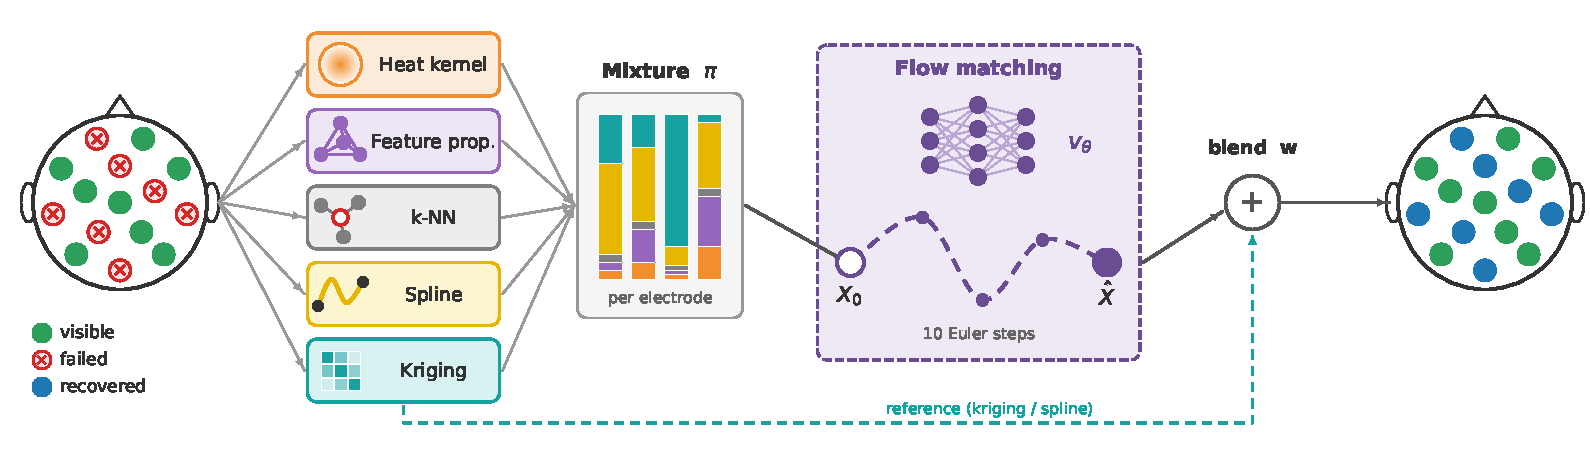
\includegraphics[width=0.9\textwidth]{anchored_flow_pipeline}
\caption{Anchored Flow. Half of the electrodes \textcolor{red}{are missing (red). Up to
five} classical estimators reconstruct them, a per-electrode mixture $\pi$
combines the estimates into the source $X_0$, flow matching transports
$X_0$ to $\hat X$ in 10 Euler steps, and the output is blended with the
kriging or spline estimate using a weight $w$ fitted on validation
participants.}
\label{fig:pipeline}
\end{figure*}

\subsection{Problem setting}

A window $X\in\mathbb{R}^{N\times R}$ contains $N$ electrodes ($N=62$ for
SEED-IV, 32 for DEAP) and $R$ time samples. For each test participant, a
fixed random half of the electrodes is hidden, simulating \textcolor{red}{missing or
failed electrodes;} a different half is drawn for each seed. The model
receives $X_{\mathrm{cond}}=M\odot X$, where the binary mask $M$ removes
the hidden electrodes, and is evaluated only on the hidden entries.
Training participants have complete montages, reflecting a laboratory that
collects full-montage data once and later \textcolor{red}{reconstructs} recordings from new
participants.

\subsection{GiFlow}

GiFlow \cite{zhang2026giflow} \textcolor{red}{uses two graphs. In the spatial graph, the
nodes are the $N$ electrodes, and two electrodes are connected when a
Gaussian kernel of their correlation distance $1-|\rho|$, computed from the
pooled recordings, exceeds 0.1. In the temporal graph, the nodes are the $R$
time samples of a window, and each sample is connected to its neighbours
(a chain). With the Laplacians $L_s$ and $L_t$ of these graphs, the
\emph{heat-kernel source}
$X_0=\exp(-\tau_sL_s)\,X_{\mathrm{cond}}\,\exp(-\tau_tL_t)$} diffuses the
observed values \textcolor{red}{to the hidden entries,} with diffusion times
$\tau_s,\tau_t$ fitted in advance. A network $v_\theta$ that alternates
spatial and temporal attention with graph message passing is then trained
by flow matching \cite{lipman2023flow} along the linear path
$X_t=(1-t)X_0+tX$, regressing the velocity $X-X_0$ on the hidden entries.
At inference, $v_\theta$ is integrated from $X_0$ in 10 Euler steps and the
observed entries are restored. Since \textcolor{red}{a source closer to the data reduces
the transport cost $\mathbb{E}\|X-X_0\|^2$ of the flow \cite{zhang2026giflow},}
a more accurate source is expected to improve the result. \textcolor{red}{We use our own
implementation of GiFlow.}

\textcolor{red}{Applied to EEG SR, this design has three limitations. (i)~If the
evaluation mask is} applied to entire recordings, the \textcolor{red}{hidden electrodes are}
also hidden in all training windows and never \textcolor{red}{serve as targets. (ii)~The
heat-kernel source only averages correlated neighbours, so with half of
the electrodes missing it is far from the true signal and the transport
cost is high. (iii)~The network overfits the training participants within
a single epoch, so per-epoch validation selects the first checkpoint.}

\subsection{Anchored Flow}

\textcolor{red}{Anchored Flow (Fig.~\ref{fig:pipeline}) addresses these limitations with
three modifications.}

\textcolor{red}{\emph{Full-montage training.} All electrodes are kept visible in training
windows,} and randomly selected whole electrodes (each with probability
0.5) \textcolor{red}{are hidden} as targets. Validation and test windows retain the
evaluation mask.

\textcolor{red}{\emph{Multi-representation anchoring.}} The heat-kernel source is replaced
by a per-electrode mixture \textcolor{red}{of $K$ classical estimates $\hat X_k$,}
\begin{equation}
X_0^{(n)}=\textstyle\sum_k \pi_{nk}\,\hat X_k^{(n)},\qquad
\pi_{n\cdot}=\operatorname{softmax}(\ell_{n\cdot}),
\end{equation}
\textcolor{red}{where $\hat X_k^{(n)}$ is the $k$-th estimate of electrode $n$, $\pi_{nk}$
its mixture weight, and $\ell_{n\cdot}\in\mathbb{R}^K$ learnable logits.
The estimates represent the hidden signal in complementary ways: the heat
kernel above;} feature propagation (FP) \cite{rossi2022unreasonable}, \textcolor{red}{which
repeatedly averages over spatial-graph neighbours and resets the observed
entries (40 iterations); $k$-NN, the mean of the visible spatial-graph
neighbours; the spherical spline \cite{perrin1989spherical},} computed from
10-05 electrode positions, \textcolor{red}{with the cerebellar SEED-IV electrodes CB1/CB2
placed at I1/I2; and, optionally, covariance kriging ($K=4$ or 5).} The logits are fitted on training
windows by minimizing the transport cost on hidden entries and then
frozen, \textcolor{red}{so each electrode relies} on the estimator that suits it best.
Kriging is the best linear predictor of the hidden electrodes $h$ given
the visible electrodes $v$ \cite{cressie1993statistics},
\begin{equation}
\hat X_h=\Sigma_{hv}(\Sigma_{vv}+\lambda I)^{-1}X_v,
\end{equation}
where $\Sigma$ is the second-moment matrix of the training participants
and \textcolor{red}{$\lambda$ is $10^{-2}$ times the mean electrode variance.} Whereas the spline imposes a smoothness prior,
kriging uses the empirically observed inter-electrode correlations.

\emph{Step-level early stopping.} We validate every 25--100 steps, reduce
the learning rate to $10^{-4}$, and add weight decay ($5\times10^{-4}$)
and dropout (0.3).

Finally, the output may be blended with the spline or kriging estimate as
$w\hat X_{\mathrm{model}}+(1-w)\hat X_{\mathrm{ref}}$, where $w\in[0,1]$
is fitted by least squares on validation participants; $w$ approaches
zero when the model does not generalize to unseen participants.

\textcolor{red}{\emph{Regression control.} To isolate flow matching, the same network,
source and training protocol are used to predict $X-X_0$ in a single step
at $t=0$, and the prediction is added to $X_0$ once at inference.}

\subsection{Participant-weighted kriging}

A single pooled covariance neglects inter-individual differences in head
shape, electrode placement and anatomy. For a new participant, we compute
the correlation matrix $C_v$ of the visible electrodes and assign each
training participant $p$ the weight
\begin{equation}
\color{red}
\omega_p\propto\exp\!\big(-d_p/(T\,\mathrm{sd}(d))\big),\qquad
d_p=\|C_v-C^{(p)}_v\|_F,
\end{equation}
where \textcolor{red}{$C^{(p)}_v$ uses the same visible electrodes and $\mathrm{sd}(d)$ is
the standard deviation of $d_p$ over $p$. Kriging then uses
$\sum_p\omega_p\Sigma^{(p)}$, with $\Sigma^{(p)}$ the second-moment matrix
of participant $p$.} Only the visible
electrodes of the new participant are used, but $C_v$ is estimated from
all of their test windows; the method is therefore transductive and
requires some prior recording from the participant. A variant fits one
covariance per frequency band ($<4$, 4--8, 8--13, 13--30 and $\geq$30~Hz)
and sums the band-wise estimates. The temperature $T$ is selected on
validation participants, and the weighted covariance can also replace the
pooled covariance in the anchored source.

\section{Experiments}
\label{sec:experiments}

\textbf{Data.} SEED-IV \cite{zheng2019emotionmeter} contains 15
participants recorded with 62 channels. We use a preprocessed version
(4~s segments at 250~Hz, normalized and soft-clipped to $\pm5$), which we
band-pass filter to 0.5--75~Hz and resample to 200~Hz.

DEAP \cite{koelstra2012deap} contains 32 participants with 32 EEG
channels. From the raw BioSemi recordings, we apply an average reference,
band-pass filter to 0.5--75~Hz, resample to 200~Hz and extract 60 evenly
spaced 5~s segments per participant. \textcolor{red}{As} amplitudes differ by two orders
of magnitude across participants, each recording is centred per channel,
scaled by \textcolor{red}{one} factor (preserving its topography) and soft-clipped with
$5\tanh(x/5)$, \textcolor{red}{as for SEED-IV.}

Both datasets are divided into non-overlapping 100-sample windows (at most
\textcolor{red}{15{,}000 in total, evenly subsampled).} Participants 7, 10 and 15 are held out for testing and 6 and 12
for validation; the remainder are used for training. Signals are
standardized using training statistics.

\textbf{Metrics.} NMSE is the squared error summed over all hidden entries,
divided by their total energy; Pearson correlation (PCC) is \textcolor{red}{additionally
given for the spline and kriging.} Results are given as mean $\pm$
population standard deviation over seeds 0, 1 and 2. The NMSE definition
is consequential: averaging per window and channel instead emphasizes
low-power channels and \textcolor{red}{at least} doubles the spline's NMSE on our data
(0.14 to \textcolor{red}{0.30 for seed 0).}

\textbf{Implementation.} Hidden size 64, four propagation layers, batch
size 32, Adam with EMA weights; Kaggle T4 GPUs for SEED-IV and an RTX
4050 for DEAP. All quantities other than network weights (mixture logits,
blend weight and kriging temperature) are fitted on training or
validation data only.

\section{Results}
\label{sec:results}

\begin{table}[t]
\centering
\small
\caption{NMSE (lower is better) for 50\% electrode loss on held-out
participants, mean $\pm$ SD over 3 seeds. Learned models \textcolor{red}{other than
published GiFlow} are blended with their reference estimate. --: not evaluated.}
\label{tab:main}
\setlength{\tabcolsep}{3pt}
\begin{tabular}{@{}lcc@{}}
\toprule
Method & SEED-IV & DEAP\\
\midrule
\multicolumn{3}{@{}l}{\emph{Interpolation (no training)}}\\
$k$-NN & 0.291 $\pm$ 0.007 & 0.946 $\pm$ 0.084\\
Feature propagation & 0.322 $\pm$ 0.008 & 0.829 $\pm$ 0.081\\
Spherical spline & 0.150 $\pm$ 0.006 & 0.981 $\pm$ 0.156\\
Kriging, pooled & 0.127 $\pm$ 0.010 & 0.548 $\pm$ 0.060\\
Kriging, participant-weighted & 0.116 $\pm$ 0.009 & 0.532 $\pm$ 0.056\\
\quad per frequency band & \textbf{0.114} $\pm$ 0.008 & --\\
\midrule
\multicolumn{3}{@{}l}{\emph{Learned}}\\
GiFlow, published hyperparam. & 0.335 $\pm$ 0.018 & 1.660 $\pm$ 0.975\\
Anchored Flow, spline source & 0.136 $\pm$ 0.007 & 0.677 $\pm$ 0.058\\
Regression control (no flow) & 0.133 $\pm$ 0.008 & 0.623 $\pm$ 0.032\\
Anchored Flow, + kriging & 0.127 $\pm$ 0.010 & 0.543 $\pm$ 0.053\\
\quad participant-weighted & 0.116 $\pm$ 0.009 & \textbf{0.527} $\pm$ 0.050\\
SRG-style flow, + kriging & 0.127 $\pm$ 0.010 & --\\
\bottomrule
\end{tabular}
\end{table}

\begin{table}[t]
\centering
\small
\caption{Ablation on SEED-IV, adding one modification at a time to GiFlow
with published hyperparameters (NMSE of the model alone and \textcolor{red}{blended
with FP in the first modified row and with the spline} thereafter).}
\label{tab:ablation}
\setlength{\tabcolsep}{4pt}
\begin{tabular}{@{}lcc@{}}
\toprule
Configuration & Model & Blend\\
\midrule
Published hyperparameters & 0.3350 & --\\
+ full montage, mixed source & 0.2381 & 0.2196\\
+ spline in the mixture & 0.1511 & 0.1452\\
+ validate every 100 steps & 0.1507 & 0.1450\\
+ learning rate $10^{-4}$ & 0.1405 & 0.1394\\
+ weight decay, dropout & 0.1367 & 0.1357\\
+ validate every 25 steps & 0.1364 & 0.1346\\
\bottomrule
\end{tabular}
\end{table}

\textbf{Baseline GiFlow.} With its published hyperparameters, \textcolor{red}{the} GiFlow
implementation attains an NMSE of 0.335 on SEED-IV (Table~\ref{tab:main}),
more than twice that of the spline (0.150) and higher than that of
$k$-NN. When the source mixture is learned, the heat kernel receives \textcolor{red}{at most
11\%} of the weight.

\textbf{Effect of the modifications.} Table~\ref{tab:ablation} reports the
modifications cumulatively. Full-montage training with a mixed source
\textcolor{red}{(heat kernel, FP and $k$-NN)} reduces NMSE by 29\%, and including the spline in the mixture, where it
receives 54--56\% of the weight, yields a further 37\% reduction.
Step-level validation alone has no effect, but combined with a lower
learning rate and regularization it moves the best checkpoint to 25--125
steps, and the model alone then outperforms the spline on all three seeds
(0.1335, 0.1463 and 0.1303 vs 0.1482, 0.1576 and 0.1430). \textcolor{red}{The
spline-anchored flow in Table~\ref{tab:main} uses the weight-decay
configuration (0.1357).}

\textbf{Contribution of flow matching.} \textcolor{red}{The regression control
(Table~\ref{tab:main}) achieves 0.133 blended and 0.137 alone,} matching
the flow.

\textbf{Kriging.} Pooled kriging attains 0.127 without any training, and
participant weighting reduces this to 0.116 (PCC 0.940 vs 0.925 for the
spline), below every learned \textcolor{red}{model without kriging in its source.} Band-wise covariances give 0.114,
although the variant preferred on validation attains 0.120. When kriging is included in the anchored \textcolor{red}{source
(Anchored Flow, + kriging),} it receives 99\% of the mixture weight, and
the flow performs no better than kriging alone (0.127 vs 0.127, and 0.116
vs 0.116 with participant weighting). The validation-fitted blend weights
(0, 0 and 0.30) confirm that the network learns no correction that
generalizes to new participants. \textcolor{red}{The SRG-style flow, with SRGDiff residual
guidance \cite{liu2026srgdiff}, gives the same} result.

\textbf{DEAP.} On the sparser 32-electrode montage, the spline performs
close to the trivial zero predictor (0.981, PCC 0.55), whereas kriging
reaches 0.548, and 0.532 with participant weighting (PCC 0.69). GiFlow
with published hyperparameters again underperforms the spline and is
unstable across seeds (0.980, 0.961 and 3.04). The spline-anchored flow
improves on the spline by 31\%, but validation selected the initial or
step-100 weights in all three seeds, so the gain is attributable mainly
to the source mixture (spline 39--43\%, FP 32--33\%, heat kernel
21--24\%). The regression control, which continued to improve for longer,
performs better (0.623). With kriging in the source, the flow remains
within 1\% of kriging alone.

\section{Discussion}
\label{sec:discussion}

Our results lead to three observations. First, protocol choices affected
GiFlow more than any architectural change: a training mask that hid the
evaluated electrodes and per-epoch early stopping each cost more than any
model modification we tested. Second, the source matters more than the
generative model, as the anchored source accounts for most of the
improvement and a network without flow matching performs equally well.
Third, the spherical spline is an insufficient reference: a kriging
predictor based on training covariances, weighted towards participants
similar to the new one, \textcolor{red}{matched or} outperformed every learned model on
both datasets.
\textcolor{red}{Future work should evaluate settings in which flow models may still be
advantageous, such as contiguous} missing regions, very sparse montages and
generative uses such as uncertainty estimation, \textcolor{red}{and should reproduce}
published diffusion models under \textcolor{red}{the same} protocol.

\section{Conclusion}
\label{sec:conclusion}

Anchoring GiFlow to classical estimates, training on the full montage and
applying step-level early stopping reduced its error by 59\% \textcolor{red}{on SEED-IV} and allowed
it to outperform the spherical spline on unseen participants. However, an
equivalent network without flow matching performs equally well, and
participant-weighted kriging performs better on both SEED-IV and DEAP. We
recommend that studies of learned EEG \textcolor{red}{SR} report such linear baselines
under a common error definition.

\section{Compliance with ethical standards}
\label{sec:ethics}

This study used only public datasets \cite{zheng2019emotionmeter,koelstra2012deap};
ethical approval was not required.

\section{Acknowledgments}
\label{sec:acknowledgments}


\begin{thebibliography}{9}

\bibitem{bigdely2015prep}
N.~Bigdely-Shamlo et~al.,
``The PREP pipeline: standardized preprocessing for large-scale EEG
analysis,'' \emph{Front. Neuroinform.}, vol.~9, p.~16, 2015.

\bibitem{perrin1989spherical}
F.~Perrin et~al.,
``Spherical splines for scalp potential and current density mapping,''
\emph{Electroencephalogr. Clin. Neurophysiol.}, vol.~72, no.~2,
pp.~184--187, 1989.

\bibitem{svantesson2021virtual}
M.~Svantesson et~al.,
``Virtual EEG-electrodes: Convolutional neural networks as a method for
upsampling or restoring channels,'' \emph{J. Neurosci. Methods},
vol.~355, p.~109126, 2021.

\bibitem{liu2026srgdiff}
H.~Liu, L.~Zhou, Z.~Yang, and C.~Yao,
``Step-aware residual-guided diffusion for EEG spatial super-resolution,''
in \emph{Proc. ICLR}, 2026.

\bibitem{zhang2026giflow}
Z.~Zhang, A.~Einizade, J.~H. Giraldo, and O.~Fink,
``Spatiotemporal imputation with graph-informed flow matching,''
arXiv:2606.06682, 2026.

\bibitem{lipman2023flow}
Y.~Lipman et~al.,
``Flow matching for generative modeling,''
in \emph{Proc. ICLR}, 2023.

\bibitem{zheng2019emotionmeter}
W.-L. Zheng et~al.,
``EmotionMeter: A multimodal framework for recognizing human emotions,''
\emph{IEEE Trans. Cybern.}, vol.~49, no.~3, pp.~1110--1122, 2019.

\bibitem{koelstra2012deap}
S.~Koelstra et~al.,
``DEAP: A database for emotion analysis using physiological signals,''
\emph{IEEE Trans. Affect. Comput.}, vol.~3, no.~1, pp.~18--31, 2012.

\bibitem{rossi2022unreasonable}
E.~Rossi et~al.,
``On the unreasonable effectiveness of feature propagation in learning on
graphs with missing node features,''
in \emph{Proc. LoG}, 2022.

\bibitem{cressie1993statistics}
N.~A.~C. Cressie, \emph{Statistics for Spatial Data}, Wiley, 1993.

\end{thebibliography}

\end{document}
